\chapter{Experiment and Results}
\label{ch5_Experiment_and_Results}

This chapter implements OpenCL standard for CPU and FPGA as a target device in Zynq platform. This includes POCL software framework for CPU and integration of OpenCL drivers to POCL for FPGA using xillybus. Data transfer OpenCL APIs are profiled and tested using OpenCL host application.

\section{Methodology}
The ‘basic’ device layer of POCLv0.11 is configured to use the xillybus for data transport. The customized POCL is compiled in host system. Then the POCL library is installed with required dependencies in Xillinux Distribution on Zedboard. This library implements OpenCL for CPU and OpenCL drivers for FPGA. Programmable logic contains xillybus demo bundle IP core that loopback the input data into output FIFO buffer. The OpenCL Host application has a single kernel function which performs vector addition for ‘N’ number of inputs. The data transfer APIs for FPGA device with OpenCL standard can be tested and compared with CPU's OpenCL Implementation for different N samples of data, where each sample has 32 bit data.

The main aim of this experiment is to profile the data transfer APIs for FPGA and CPU. For, CPU we have full implemented OpenCL ‘pthread’ device. As FPGA device in POCL has data transfer support, kernel function is added to the hardware logic. Xillybus demo bundle can be customized with the kernel function logic. The xillydemo project is opened using TCL script in Vivado design suite. In the interface file, we introduce the kernel logic between input and output buffers. Then it is necessary to run the implementation and generate bitstream file. This process can be referred to section 4.3. The new bitstream file is copied to boot partition of SD card and Zedboard is booted with the xillybus bitstream.
 
\section{Adding Xillybus device in POCL Framework}
The ‘basic’ device in POCL can be used for POSIX compliant device. But this device layer is customized for a new hardware. The following are the key points about the ‘basic’ device layer and changes introduced for xillybus device,
\begin{itemize}
	\item pocl\_device\_ops structure contains all the necessary function pointers for hardware related function calls. Here, we update the device name as “xillybus”. 
	\item \_cl\_device\_id structure contains hardware related information like number of compute units, device type, maximum work group size, global memory, local memory etc.,
	\item If an accelerator is attached to the xillybus, we can update the device type as CL\_DEVICE\_TYPE\_ACCELERATOR.
	\item The pocl\_basic\_probe() validates the environmental variable and the device name. If both the name matches, the hardware implementation of ‘basic’ is accounted or else pthread is used.
	\item The POCL initialization function, pocl\_basic\_init() updates the compute unit and other memory initialization.
	\item The memory allocation functions for POCL will copy the host pointer address as a new memory location inside the device layer, which is like a ‘pthread’ devices.
	\item The pocl\_basic\_read and pocl\_basic\_write are hardware data transfer APIs. By default, Basic device copies the host pointer address for both write and read operation as shown in below code snippet.
	\lstinputlisting[firstline=25, lastline=28, frame=none, numbers=left, basicstyle=\fontsize{11}{11}\selectfont\ttfamily, backgroundcolor=\color{gainsboro}]{code_snippet.txt}
	\item For FPGA device, we have xillybus host Linux device driver as an OpenCL driver. In read and write data transfer APIs, Named pipes are used for streaming data between Processing system and Programming Logic.
	\item We open a file pointer for /dev/xillybus\_read\_32 in Read only mode and data is read to host pointer for given size.
	\lstinputlisting[firstline=30, lastline=34, frame=none, numbers=left, basicstyle=\fontsize{11}{11}\selectfont\ttfamily, backgroundcolor=\color{gainsboro}]{code_snippet.txt}
	\item Also, we open a file pointer for /dev/xillybus\_write\_32 in Write only mode and data is written to the host pointer for given size.
	\lstinputlisting[firstline=36, lastline=40, frame=none, numbers=left, basicstyle=\fontsize{11}{11}\selectfont\ttfamily, backgroundcolor=\color{gainsboro}]{code_snippet.txt}
\end{itemize}

\section{Installing POCL}
\subsection{Github location to install POCL}
The below url has the softwares and packages required to install POCL.

\url{https://github.com/abisheksethu/opencl-implementation}

\subsection{Installation method}
POCL-0.11 software package can be installed on Xillinux distribution. To install pocl-0.11, we need following dependencies to be installed before POCL compilation. 
\begin{enumerate}
	\item LLVM compiler infrastructure and other LLVM sub projects likes Clang and compiler-rt are required for POCL’s kernel compiler. It is available as both source code and pre-compiled binaries. LLVM-3.6 version requires host C++ toolchain version to be greater than 4.7. 
	\item Cmake package controls the compilation flow of a software using simple platform and compiler independent configuration file. We use cmake-3.7 to generate native makefiles and workspace that can be used in compiler environment. 
	\item OpenCL Installable Client Driver, ocl-icd allows multiple OpenCL Implementation for a same system that can co-exist. The OpenCL ICD loader library allows the host application to choose a platform from the installed platform and redirect the API calls to the respective platform. The POCL can be compiled with or without ICD loader. We compile using OCL ICD 2.2.10 version which is available as a source code. So, we need to compile and install the ICD loader on host System.
	\item Other dependencies like libhwloc-dev 1.8, libz-dev, libffi-dev, autoconf, libtool, ruby1.8-dev, libtinfo-dev are also installed on the host platform
	\item To profile the data transfer APIs for CPU and FPGA, we install Performance Application Programming Interface, PAPI libraries. This library 	enables the software engineer to analyze the relation between software performance with hardware in near real time.
\end{enumerate}

This work has been maintained in git hub repository under the project name opencl-implementation. It can be cloned from the above mentioned Github location. The project contains all the necessary dependency packages, poclv0.11 and host application. The POCL’s basic layer has been customized for a new xillybus device with data transfer APIs. It also contains install script that installs all the packages and POCL. When we customize POCL software framework, POCL package can be compiled and installed separately using generated makefiles, which is available inside pocl-0.11/build sub-directory of the project.

\section{Host Application for CPU and FPGA}
The OpenCL host application performs vector addition on a given platform. This application is developed using OpenCL C APIs that can execute on different type of device. The kernel function is written with the file extension of .cl. The kernel performs addition of two same input value and store the output in a vector form. The host application is executed on Zedboard using pocl OpenCL library for CPU and FPGA devices. The application code is compiled using GCC, GNU Compiler Collection with POCL’s dynamic library and PAPI’s static library. The host application executes on CPU using ‘pthread’ device layer, while it executes on FPGA using ‘xillybus’, which is a customized 'basic' device layer that has been patched for FPGA data transfer APIs. 
 
OCL-ICD 2.2.10 has been installed in Xillinux. The POCL configuration environment detects the OCL-ICD and it enables the ICD loader option for compilation. When the host OpenCL application executes, the available platforms should be available in the ICD loader file. The ICD loader file contains the path of the opencl-implementation. After installation of POCL, Path of POCL library is added to the ICD loader file which is available at /etc/OpenCL/vendors/pocl.icd location. This configuration has been included at the end of install script.

The kernel function used in the host application is shown in code snippet. For superscalar architecture, this function can be executed by unrolling the parallel region of the kernel code such that all the work items are statically assigned to the multiple functional units. The call to get\_global\_id() returns the index of the current work item from global index space. Here the index of the work item matches with the buffer index. The main difference to C notation standard is the kernel function uses the global qualifier in the kernel arguments. 
	\lstinputlisting[firstline=42, lastline=47, frame=none, numbers=left, basicstyle=\fontsize{11}{11}\selectfont\ttfamily, backgroundcolor=\color{gainsboro}]{code_snippet.txt}

The OpenCL application flow is shown in the \ref{fig:1_HOA}. The OpenCL APIs which are responsible for platform level queries, memory allocation and data transfer are grouped into Platform APIs. The OpenCL APIs which are responsible to build the program and generate code for hardware are categorized into Runtime APIs. First, the application creates context based on platform and device information. Second, With the respective context, we build and generate code for kernel function. Then the queued commands starts its execution after clFinish(). The given host application is discussed in detail with code snippet.
\begin{figure}[h]
    \centering
    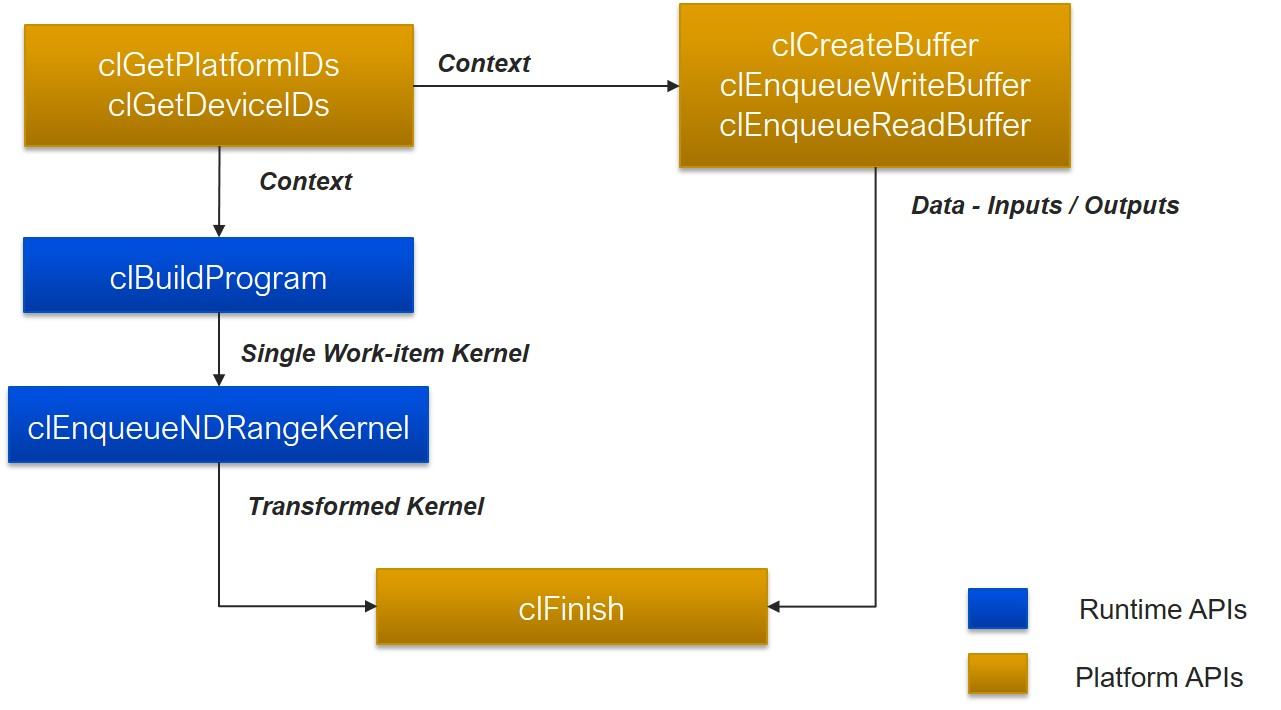
\includegraphics[width=1\textwidth]{OpenCL_APIs}
    \caption{Host Application Flow}
    \label{fig:1_HOA}
\end{figure}

\begin{itemize}
	\item The available number of platforms and its information are requested. The device ID can be obtained for a device with given device type. We have two types of device which is CPU and FPGA. This application receives device ID of any type, which is passed as a reference in the argument.
	\lstinputlisting[firstline=48, lastline=54, frame=none, numbers=left, basicstyle=\fontsize{11}{11}\selectfont\ttfamily, backgroundcolor=\color{gainsboro}]{code_snippet.txt}
	\item A context is created from the device\_id. This context has been used for entire access to the device. 
	\item There are two possible ways to load the kernel function. If we have the binary source for a kernel function, it can create the program using clCreateProgramwithBinary() function. On other hand, kernel function with .cl extension must be loaded using the source code. Then the kernel source is created using clCreateProgramwithSource(). 
	\item The key conversion of kernel function into compute kernel part is provoked by clBuildProgram() function call. Here the work item is created with LLVM Intermediate Representation. These work-item does not contain any kernel arguments or work group information. 
	\lstinputlisting[firstline=56, lastline=61, frame=none, numbers=left, basicstyle=\fontsize{11}{11}\selectfont\ttfamily, backgroundcolor=\color{gainsboro}]{code_snippet.txt}
	\item The kernel arguments for each work item is created using clSetKernelArg(). Here, the arguments are called as input and output. 
	\item A command queue is created, where the write, read and execute commands are enqueued. First Write command is enqueued using clEnqueueWriteBuffer(). The input data array is passed as one of the arguments to the function.
	\lstinputlisting[firstline=63, lastline=68, frame=none, numbers=left, basicstyle=\fontsize{11}{11}\selectfont\ttfamily, backgroundcolor=\color{gainsboro}]{code_snippet.txt}
	\item The function clEnqueueNDRangeKernel() executes the kernel over entire range of 1D input data set. We give maximum work group size to exploit maximum parallelism for CPU. 
	\lstinputlisting[firstline=71, lastline=78, frame=none, numbers=left, basicstyle=\fontsize{11}{11}\selectfont\ttfamily, backgroundcolor=\color{gainsboro}]{code_snippet.txt}
	\item Finally, the read command is enqueued and the output data is stored in ‘results’ variable. The clFinish releases all the commands. The output data is validated from CPU and FPGA. 
\end{itemize}

The host application can be found at opencl-implementation/host\_app location in git repository. It has run script which can automate the compilation and execution environment. POCL library location is added to LD\_LIBRARY\_PATH. The execution flow is shown below.
\begin{enumerate}
	\item POCL checks for the available device in the environmental variable. This feature can be enabled by exporting the required device. First, we export ‘pthread’ device. So, the kernels are executed on CPU.
	\item Another environmental variable is updated for varied sizes of data samples. Then the host application starts its execution. This process is repeated for 1024 to 16384 samples for about 16 iterations. 
	\item Each data set is tested for 10 iterations. The timing information for all OpenCL APIs are stored in a local file.
	\item Second, we export ‘xillybus’ device to POCL\_DEVICES. Thus, the data transfers are initiated to xillybus demo bundle on FPGA and it follows step 2 and 3. As xillybus is a customized form of ‘basic’ device layer, the kernel functions are not transferred to FPGA. 
\end{enumerate}

\section{Results}
The profiling for OpenCL APIs are performed using Performance Application Programming Interface, PAPI library. The timing information is captured before and after OpenCL API calls. The kernel function and data transfers are tested for different data set samples. Each data set samples are tested for ten iterations and average time value is recorded. The timing information are measured in microseconds. For example, the current pocl device is exported as ‘pthread’ for CPU. The application is executed for 10 iterations for 1024 input vectors, where size of each input vector is 32 bit. This process is repeated up to 16384 input vectors in 16 iterations. This is also tested and profiled for xillybus device. Though the xillybus does not receive the kernel logic from POCL, we have hard coded the hardware for same kernel logic. Thus, the data read from FPGA should match the expected output. 

\subsection{HOST to DEVICE Data Transfer}
The Data transfer between host and device are analyzed using the timing values, which are recorded in the tables \ref{tab:pthread_Table} and \ref{tab:xillybus_Table} for both pthread and xillybus devices.
% Table generated by Excel2LaTeX from sheet 'REPORT'
\begin{table}[h]
  \centering
  \begin{adjustbox}{width=0.8\textwidth}
	\small
    \begin{tabular}{|c|c|c|c|}
    \toprule
    Iteration  & Number of Samples & clEnqueueWriteBuffer & clEnqueueReadBuffer \\
    \midrule
    1     & 1024  & 84.7  & 855.3 \\
    2     & 2048  & 99.4  & 877.5 \\
    3     & 3072  & 110.8 & 884.7 \\
    4     & 4096  & 123.4 & 901.2 \\
    5     & 5120  & 143.7 & 912.4 \\
    6     & 6144  & 154.7 & 912.6 \\
    7     & 7168  & 169.5 & 920 \\
    8     & 8192  & 189.7 & 934.8 \\
    9     & 9216  & 212.1 & 949.3 \\
    10    & 10240 & 200.9 & 960.3 \\
    11    & 11264 & 217.3 & 971.2 \\
    12    & 12288 & 224.8 & 986.4 \\
    13    & 13312 & 236   & 995.5 \\
    14    & 14336 & 248.7 & 1017.6 \\
    15    & 15360 & 260   & 1041.3 \\
    16    & 16384 & 271   & 1032 \\
    \bottomrule
    \end{tabular}%
    \end{adjustbox}%
	\caption{Timing Analysis for Data Transfers APIs -- 'pthread' device}
  \label{tab:pthread_Table}%
\end{table}%
% Table generated by Excel2LaTeX from sheet 'REPORT'
\begin{table}[h]
  \centering
  \begin{adjustbox}{width=0.8\textwidth}
  \small
    \begin{tabular}{|c|c|c|c|}
    \toprule
    Iteration  & Number of Samples & clEnqueueWriteBuffer & clEnqueueReadBuffer \\
    \midrule
    1     & 1024  & 119.7 & 626.6 \\
    2     & 2048  & 123.6 & 647 \\
    3     & 3072  & 136.4 & 685.7 \\
    4     & 4096  & 140.2 & 708 \\
    5     & 5120  & 147.4 & 722.4 \\
    6     & 6144  & 154.8 & 746.7 \\
    7     & 7168  & 164.1 & 783.3 \\
    8     & 8192  & 169.4 & 803.6 \\
    9     & 9216  & 178.9 & 824.1 \\
    10    & 10240 & 186   & 846.2 \\
    11    & 11264 & 191.5 & 864.6 \\
    12    & 12288 & 201   & 886.5 \\
    13    & 13312 & 206.2 & 899.7 \\
    14    & 14336 & 217.3 & 939.9 \\
    15    & 15360 & 223   & 958.5 \\
    16    & 16384 & 235.7 & 967.8 \\
    \bottomrule
    \end{tabular}%
    \end{adjustbox}%
	\caption{Timing Analysis for Data Transfers APIs -- 'xillybus' device}
  \label{tab:xillybus_Table}%
\end{table}%


\subsection{Comparison of OpenCL APIs for pthread and xillybus device}
The Timing graph for clEnqueueWriteBuffer and clEnqueueReadBuffer OpenCL APIs are shown in figure \ref{graph1:write} and \ref{graph2:read}. We observe the xillybus device data transfers are faster than pthread device, when the number of samples are increased.
%% \hfill
%	 \begin{figure}[!b]
%	 \centering 
%	 \begin{tikzpicture}[scale = 1.1]
%	 \begin{semilogyaxis}[
%		xlabel=Datasize$(N)$,
%		ylabel=Time $(ms)$,
%	 % 	scaled ticks=base 10:-5,
%	 xtick pos=left,
%	 ytick pos=left,
%	 ymax = 600,
%	 xmax = 16777216,
%	 yticklabels={1,10,100,1000},
%	 %	symbolic y coords={0.4239,0.847,1.67,3.33,6.69,13.33,26.63,54.41,70,150,290,560},
%	 %  symbolic y coords = {-1,-0.698,-0.522,-0.397,-0.301,-0.221,-0.154,-0.0969,-0.0457,0.0,0.3010,0.4771,0.6021,0.6990,0.7782,0.8450,0.9030,0.9542,1.0,1.3010,1.4771,1.6021,1.6990,1.7782,1.8450,1.9030,1.9542,2.0,2.3010,2.4771,2.6021,2.6990,2.7782,2.8452,2.9030,2.9542,3.0},
%	 %    ytick=data, 
%	 %    yticklabels={0.1,0.2,0.3,0.4,0.5,0.6,0.7,0.8,0.9,1,2,3,4,5,6,7,8,9,10,20,30,40,50,60,70,80,90,100,200,300,400,500,600,700,800,900,1000},
%	 symbolic x coords={131072,262144,524288,1048576,2097152,4194304,8388608,16777216},
%	 enlargelimits=true,
%	 xtick=data,
%	 xticklabels={$2^{17}$,$2^{18}$,$2^{19}$,$2^{20}$,$2^{21}$,$2^{22}$,$2^{23}$,$2^{24}$},
%	 width = 10cm,
%	 xmode = normal,
%	 legend pos=north west,
%	 legend style={draw=none}
%	 ] 
	 
	 
	 % \hfill
	 \begin{figure}[!b]
	 \centering 
	 \begin{tikzpicture}[scale = 1.1]
	 \begin{semilogyaxis}[
    xlabel=Number of Samples,
	ylabel=Time $(μs)$,
	 % 	scaled ticks=base 10:-5,
	 xtick pos=left,
	 ytick pos=left,
	 ymax = 300,
	 xmax = 16384,
	 %	 ymode=log,log ticks with fixed point,
	 %	grid=major,
	   %symbolic y coords={1024, 2048, 3072, 4096, 5120, 6144, 7168, 8192, 9216, 10240, 11264, 12288, 13312, 14336, 15360, 16384},
	 %   ytick={data},
	 symbolic x coords={1024, 2048, 3072, 4096, 5120, 6144, 7168, 8192, 9216, 10240, 11264, 12288, 13312, 14336, 15360, 16384},
	 xtick=data,
	 xticklabels={1024, 2048, 3072, 4096, 5120, 6144, 7168, 8192, 9216, 10240, 11264, 12288, 13312, 14336, 15360, 16384},
	 %	symbolic y coords={0.4239,0.847,1.67,3.33,6.69,13.33,26.63,54.41,70,150,290,560},
	 width = 10cm,
	 xmode = normal,
	 legend pos=north west,
	 legend style={draw=none}
	 ]    
   
	\addplot plot coordinates {
	    (1024,     84.7)
		(2048,     99.4)
		(3072,    110.8)
		(4096,    123.4)
		(5120,    143.7)
		(6144,    154.7)
		(7168,   169.5)
		(8192,   189.7)
		(9216,     212.1)
		(10240,     200.9)
		(11264,    217.3)
		(12288,    224.8)
		(13312,    236)
		(14336,    248.7)
		(15360,   260)
		(16384,   271)
		};

	\addplot plot coordinates {
	    (1024,     119.7)
		(2048,     123.6)
		(3072,    136.4)
		(4096,    140.2)
		(5120,    147.4)
		(6144,    154.8)
		(7168,   164.1)
		(8192,   169.4)
		(9216,     178.9)
		(10240,    186)
		(11264,    191.5)
		(12288,    201)
		(13312,    206.2)
		(14336,    217.3)
		(15360,   223)
		(16384,   235.7)
		};

  

%	\legend{MXP(Byte)\\Intel i3(Byte)\\ARMv7(Byte)\\Neon(Byte)\\} 
    \legend{pthread\\xillybus\\} 
	\end{semilogyaxis}
	\end{tikzpicture} 
	\label{writebuffer} 
% \hspace{4.5cm}       $f(samples,time) = a * x ^ 2 + b* x + c$
\caption{Comparison of Write buffer API} 
\label{dag:write}

\end{figure}
\begin{figure}[h!]
	 \centering 
	 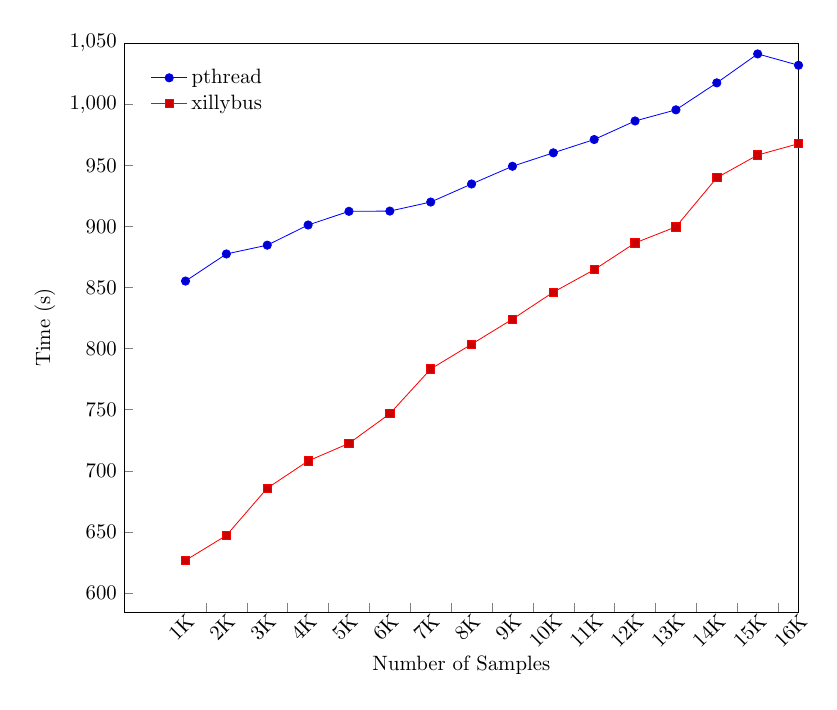
\begin{tikzpicture}[scale = 0.75]
	 \begin{axis}[
    	xlabel=Number of Samples,
		ylabel=Time ($\upmu$s),
	 	%scaled ticks=base 10:-5,
	 	xtick pos=left,
		ytick pos=left,
		ymax = 1050,
		xmax = 16384,
   		symbolic x coords={1024, 2048, 3072, 4096, 5120, 6144, 7168, 8192, 9216, 10240, 11264, 12288, 13312, 14336, 15360, 16384},
	 	xtick=data,
		xticklabels={1K, 2K, 3K, 4K, 5K, 6K, 7K, 8K, 9K, 10K, 11K, 12K, 13K, 14K, 15K, 16K},
	 	width = 13cm,
	 	xmode = normal,
	 	legend pos=north west,
	    legend style={draw=none},
	 	x tick label style={rotate=45, anchor=north east, inner sep=0mm},
		major x tick style = {opacity=0},
		minor x tick num = 1,
		minor tick length=1ex,
		every node near coord/.append style={
        anchor=west,
        rotate=90,
        font=\tiny
		},
	 ]    
   
	\addplot plot coordinates {
	    (1024,     855.3)
		(2048,     877.5)
		(3072,     884.7)
		(4096,     901.2)
		(5120,     912.4)
		(6144,     912.6)
		(7168,     920)
		(8192,     934.8)
		(9216,     949.3)
		(10240,    960.3)
		(11264,    971.2)
		(12288,    986.4)
		(13312,    995.5)
		(14336,    1017.6)
		(15360,    1041.3)
		(16384,    1032)
		};
    
	\addplot plot coordinates {
	    (1024,     626.6)
		(2048,     647)
		(3072,     685.7)
		(4096,     708)
		(5120,     722.4)
		(6144,     746.7)
		(7168,     783.3) 
		(8192,     803.6)
		(9216,     824.1)
		(10240,    846.2)
		(11264,    864.6)
		(12288,    886.5)
		(13312,    899.7)
		(14336,    939.9)
		(15360,    958.5)
		(16384,    967.8)
		};
		
    \legend{pthread\\xillybus\\} 
	\end{axis}
	\end{tikzpicture} 
	\label{writebuffer} 
	\caption{Timing Analysis for clEnqueueReadBuffer API} 
	\label{graph2:read}
\end{figure}